% Updated Sept 26
\begin{figure}[t]
\centering
\begin{minipage}[b]{0.48\textwidth}
\centering
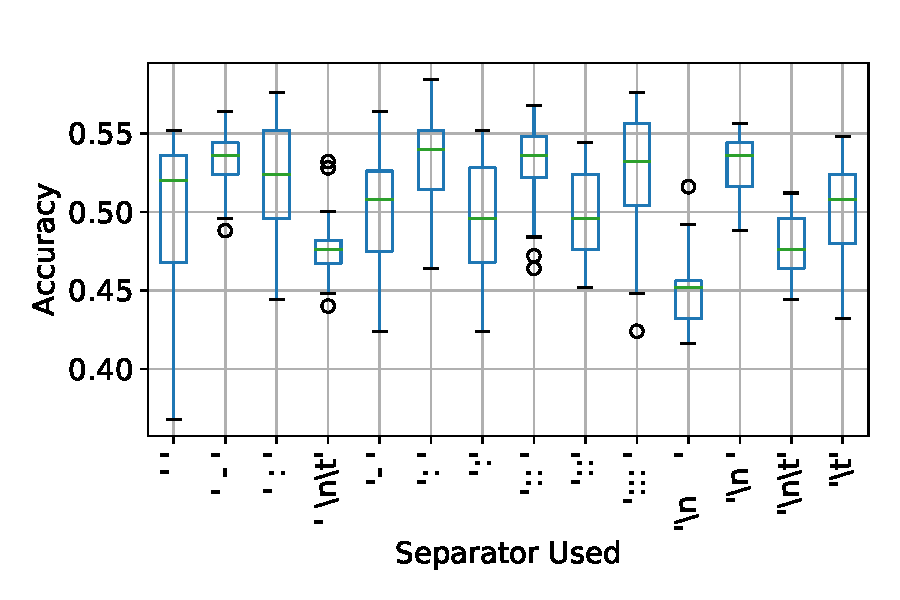
\includegraphics[width=\linewidth]{figures/paperboxplot_by_feature_value_rankscore_2_task1283_Llama-2-7b-hf.pdf}
\caption{Example of accuracy variance for different choices of constants in $\mathcal{S}_1$ for task1283.}\label{fig:example_boxplot_constant}
\end{minipage}\hfill
\begin{minipage}[b]{0.48\textwidth}
\centering
\footnotesize
\captionsetup{type=table} %% tell latex to change to table

%\begin{tabular}{@{}ccc@{}}
%\toprule
%\multirow{2}{*}{\begin{tabular}[c]{@{}c@{}}Constant\\ Set\end{tabular}} & \multicolumn{2}{c}{\begin{tabular}[c]{@{}c@{}}Tasks with differently\\performing constants\end{tabular}} \\ \cmidrule(l){2-3} 
%                                                                        & Weak Diff.                                          & Strong Diff.                                          \\ \midrule
%$\mathcal{C}$                       & 22\%                     & 0\%                        \\
%$\mathcal{S}_1$                    & 42\%                     & 18\%                       \\
%$\mathcal{S}_2$ & 0\%                      & 0\%                        \\
%$\mathcal{F}_{item1}$ % chosen\_item\_wrapper
%& 0\%                      & 0\%                        \\
%$\mathcal{F}_{item2}$ %chosen\_number\_format              
%& 57\%                     & 57\%                       \\
%$\mathcal{F}_{casing}$                 & 5\%                      & 0\%                        \\ \bottomrule
%\end{tabular}

\caption{Tasks where at least two constants yield different performance (\textit{weakly} different if their boxes in a boxplot do not overlap, \textit{strongly} if boxes including whiskers do not overlap).
}\label{tab:percentage_tasks_different}
\begin{tabular}{cccc}
\toprule
                                     & \begin{tabular}[c]{@{}c@{}}Median Spread\\ (range {[}0, 1{]})\end{tabular} & \begin{tabular}[c]{@{}c@{}}Weak \\ Diff. \end{tabular} & \begin{tabular}[c]{@{}c@{}}Strong \\ Diff.\end{tabular} \\ \midrule

$\mathcal{C}$           & 0.144                                                   & 29\%                                                    & 1\%                                                                                                                          \\
$\mathcal{S}_1$          & 0.132                                               & 43\%                                                    & 22\%                                                                                                                          \\
$\mathcal{S}_2$             & 0.238                          & 0\%                                                     & 0\%                                                                                                                          \\
$\mathcal{F}_{\text{item1}}$       & 0.176                                            & 0\%                                                     & 0\%                                                                                                                            \\  % wrapper
$\mathcal{F}_{\text{item2}}$           & 0.173                                         & 45\%                                                    & 10\%                                                                                                                           \\ % format
$\mathcal{F}_{\text{casing}}$              & 0.188                                           & 3\%                                                     & 0\%                                                                                                                         \\ \bottomrule
\end{tabular}
\vspace*{0.1cm}

\end{minipage}
\end{figure}
\begin{comment}
    \begin{figure}[t]
\centering
\begin{minipage}[b]{0.48\textwidth}
\centering
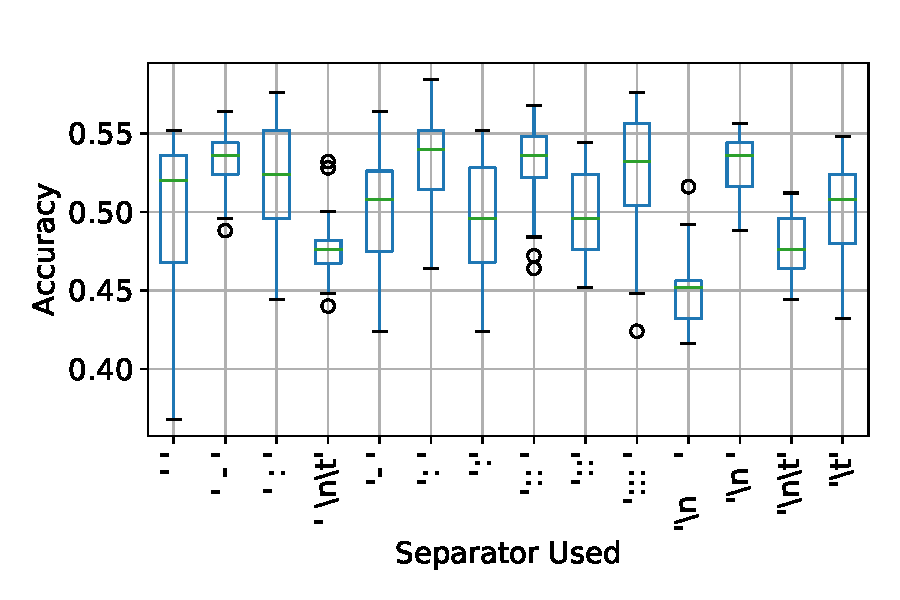
\includegraphics[width=\linewidth]{figures/paperboxplot_by_feature_value_rankscore_2_task1283_Llama-2-7b-hf.pdf}
\caption{Example of accuracy variance for different choices of constants in $\mathcal{S}_1$ for task1283.}\label{fig:example_boxplot_constant}
\end{minipage}\hfill
\begin{minipage}[b]{0.48\textwidth}
\centering
\footnotesize
\captionsetup{type=table} %% tell latex to change to table

%\begin{tabular}{@{}ccc@{}}
%\toprule
%\multirow{2}{*}{\begin{tabular}[c]{@{}c@{}}Constant\\ Set\end{tabular}} & \multicolumn{2}{c}{\begin{tabular}[c]{@{}c@{}}Tasks with differently\\performing constants\end{tabular}} \\ \cmidrule(l){2-3} 
%                                                                        & Weak Diff.                                          & Strong Diff.                                          \\ \midrule
%$\mathcal{C}$                       & 22\%                     & 0\%                        \\
%$\mathcal{S}_1$                    & 42\%                     & 18\%                       \\
%$\mathcal{S}_2$ & 0\%                      & 0\%                        \\
%$\mathcal{F}_{item1}$ % chosen\_item\_wrapper
%& 0\%                      & 0\%                        \\
%$\mathcal{F}_{item2}$ %chosen\_number\_format              
%& 57\%                     & 57\%                       \\
%$\mathcal{F}_{casing}$                 & 5\%                      & 0\%                        \\ \bottomrule
%\end{tabular}

\caption{Tasks where at least two constants yield different performance (\textit{weakly} different if their boxes in a boxplot do not overlap, \textit{strongly} if boxes including whiskers do not overlap).
}\label{tab:percentage_tasks_different}
\begin{tabular}{cccc}
\toprule
                                     & \begin{tabular}[c]{@{}c@{}}Median Spread\\ (range {[}0, 1{]})\end{tabular} & \begin{tabular}[c]{@{}c@{}}Weak \\ Diff. \end{tabular} & \begin{tabular}[c]{@{}c@{}}Strong \\ Diff.\end{tabular} \\ \midrule

$\mathcal{C}$           & 0.156                                                   & 28\%                                                    & 2\%                                                                                                                          \\
$\mathcal{S}_1$          & 0.152                                               & 48\%                                                    & 27\%                                                                                                                          \\
$\mathcal{S}_2$             & 0.246                          & 0\%                                                     & 0\%                                                                                                                          \\
$\mathcal{F}_{item1}$       & 0.209                                            & 0\%                                                     & 0\%                                                                                                                            \\
$\mathcal{F}_{item2}$           & 0.219                                         & 43\%                                                    & 7\%                                                                                                                           \\
$\mathcal{F}_{casing}$              & 0.197                                           & 5\%                                                     & 0\%                                                                                                                         \\ \bottomrule
\end{tabular}
\vspace*{0.1cm}

\end{minipage}
\end{figure}
\end{comment}